\documentclass{article}
\usepackage{graphicx}
\usepackage{float}
\usepackage[acronym]{glossaries}
\usepackage{fullpage}

\loadglsentries{acronyms}
\makeglossaries

\begin{document}

\begin{tabular}{rl}
  \textbf{Lab 8:} & DC Generators \\
  \textbf{Performed:} & March 26, 2013 \\
  \textbf{Partners:} & Rawley Dent \\ & Charles Pittman \\
  \textbf{Instructor:} & Dr. Weatherford
\end{tabular}

%\setlength\parindent{0pt}

\section*{Abstract}

In this experiment, the basic principles of operation of DC generators were
studied. The output voltage ($V_T$) and output current current ($I_L$)
relationship for separately excited, shunt, and compound generators were
studied under various loads.

\section*{Results}

\begin{figure}[H]
  \centering
    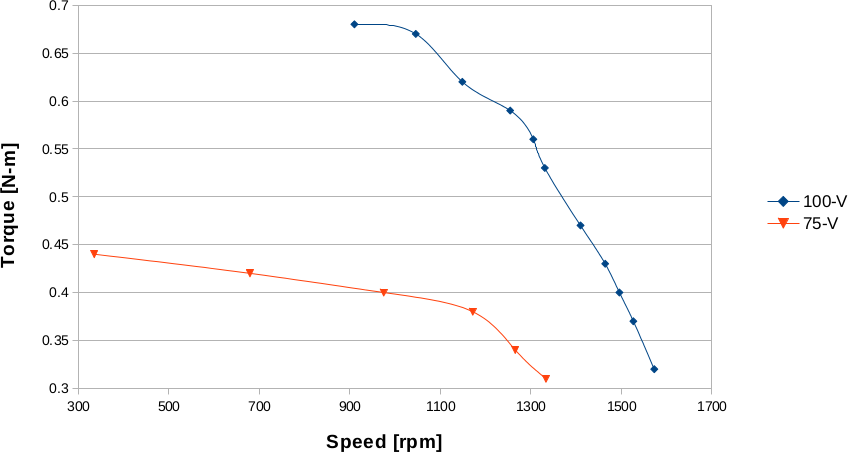
\includegraphics[width=0.7\textwidth]{img/graph}
    \caption{\textbf{Comparison of Terminal Characteristics}}
    \label{fig:graph}
\end{figure}

\section*{Conclusions}

The terminal characteristics for DC motors are induced torque and speed; for DC
generators they are terminal voltage and line current.  Figure~\ref{fig:graph}
shows a comparison of the terminal characteristics of a separately excited,
shunt, and compound generators.

The terminal characteristics of a separately excited generator are linear,
following $V_T = E_A - {I_A}{R_A}$.  As the load increased, the line and
armature currents ($I_L$ and $I_A$) increased, decreasing $V_T$, as the internal
generated voltage ($E_A$) is independent of $I_A$.

A shunt generator behaves similarly, except that the field current ($I_F$) is
proportional to $V_T$.  As $I_F$ decreases $V_T$, flux, and $E_A$ also
decrease. This causes $I_A$ to increase, which decreases $V_T$ further, so the
relationship is not quite linear.

The terminal characteristics of a compound generator consist of two opposing
terminal voltages, following $V_T = E_A - I_A(R_A + R_S)$.  As the load
increased, $I_L$ and $I_A$ increased.  Since $I_A$ increases, the total
magneto-motive force increases, which increases the flux, which increases
$E_A$, which increases $V_T$.

\end{document}
